\documentclass{article}
\usepackage{graphicx} % Required for inserting images
\usepackage{amsmath}
\usepackage[margin=.5in]{geometry}
\usepackage{float}
\setlength{\parindent}{0pt}

\title{Homework 9}
\author{Quan Nguyen}
\date{May 2026}

\begin{document}

\maketitle
See https://github.com/nguyencquan/Markov2026 for code used in simulations.
\section{Cargo delivery along an actin Filament}
Actin transport from the nucleus at $i=0$ to the membrane at $i=L$. Assume an 
increase rate of $\alpha > 1$ and a decrease rate of $\beta \geq 0$. Note
L is an absorbing state and $i=0$ is a reflective state. Let $T = \text{inf}_{t\geq0}\{t:X_{t}=L\}$
be the delivery time until state L is reached and $m_{i} = E[T|X(0)=i]$ be
the mean delivery time starting from node i.

\textbf{a)}

\begin{align}
m_{i} &= \text{Expected time at i + expected time spent after jump}\\
&= \frac{1}{\lambda_{i}} + \sum_{j=1}^{L} E[\text{T after jumping to j| jumped to j}]P(\text{Jumping to j})\\
&= \frac{1}{\lambda_{i}} + \sum_{j=1}^{L} m_{j} \frac{q(i,j)}{\lambda_{i}}
\end{align}

This is mostly a general scenerio without boundary conditions
 so a more nicely fleshed out variation:

\begin{equation}
m_{i} = \begin{cases}
    \frac{1}{\alpha} + m_{1},& i = 0\\
    \frac{1}{\alpha+\beta} + m_{i-1} \frac{\beta}{\alpha+\beta} + m_{i+1} \frac{\alpha}{\alpha+\beta},& 0<i<L\\
    0,& i= L
\end{cases}
\end{equation}

\textbf{b)}
If we assume an unbiased case, let us replace beta with alpha for simplicity:
\begin{equation}
m_{i} = \begin{cases}
    \frac{1}{\alpha} + m_{1},& i = 0\\
    \frac{1}{2\alpha} + \frac{1}{2} (m_{i-1} + m_{i+1}),& 0<i<L\\
    0,& i= L
\end{cases}
\end{equation}


\begin{align}
m_{0} &= \frac{1}{\alpha} + m_{1}\\
&= \frac{1}{\alpha} + \left(\frac{1}{2\alpha} + \frac{1}{2}(m_{0} + m_{2})\right)\\
&= \frac{3}{\alpha} + m_{2}= \frac{3*2}{2\alpha} + m_{2}\\
&= \frac{3}{\alpha} + \left(\frac{1}{2\alpha} + \frac{1}{2}(m_{1} + m_{3})\right) = \frac{3}{\alpha} + \left(\frac{1}{2\alpha} + \frac{1}{2}(m_{0} - \frac{1}{\alpha} + m_{3})\right)\\
&= \frac{6}{\alpha} + m_{3}= \frac{4*3}{2\alpha} + m_{3}\\
&=\frac{6}{\alpha} + \left(\frac{1}{2\alpha} + \frac{1}{2}(m_{2} + m_{4})\right) = \frac{6}{\alpha} + \left(\frac{1}{2\alpha} + \frac{1}{2}(m_{0} - \frac{3}{\alpha} + m_{4})\right)\\
&= \frac{10}{\alpha} + m_{4} = \frac{5*4}{2\alpha} + m_{4}\\
&=...\\
&= \frac{L(L+1)}{2\alpha} + m_{L} = \frac{L(L+1)}{2\alpha}
\end{align}

To prove that this actually works through the use of induction.
We test the base case for $m_{0} = \frac{3*2}{2\alpha} + m_{2}$ and this is true
as per the equatoin above. Now let us assume that for all $ 1 < i\leq k$
$m_{0} = \frac{(i)(i+1)}{2\alpha} + m_{i}$, we will prove that $k+1$ is also true assuming
$k < L$
\begin{align}
m_{0} &= \frac{(k)(k+1)}{2\alpha} + m_{k} =\frac{(k)(k+1)}{2\alpha} + \left(\frac{1}{2\alpha} + \frac{1}{2}(m_{k-1} + m_{k+1})\right)\\
&= \frac{(k)(k+1)}{2\alpha} + \left(\frac{1}{2\alpha} + \frac{1}{2}(m_{0}-\frac{(k)(k-1)}{2\alpha} + m_{k+1})\right)\\
&= \frac{2(k)(k+1)}{2\alpha} + \left(\frac{2}{2\alpha} -\frac{(k)(k-1)}{2\alpha} + m_{k+1}\right)\\
&= \frac{k[2(k+1) - (k-1)]+2}{2} + m_{k+1} = \frac{k^{2}+3k+2}{2\alpha} + m_{k+1}\\
&= \frac{(k+2)(k+3)}{2\alpha}+ m_{k+1}
\end{align}

Essentially this means that the rate that the transport goes forward and backward is
the same. Hence this kind of transport is pretty much diffusion which has a quadratic relationship to distance.
And when transport backwards and forward is the same, it takes on average
$\frac{L(L+1)}{2\alpha}$ to get to the membrane.

\textbf{c)}
I think $M_{0}$ will depend probably just linearly on L. I think my reaosning is that
we can combine both the alpha and beta value and see that the expected
jump distance is a positive constant. Hence the scaling between distance and time should be linear.

Notice that the equation for detailed balance can be treated as a linear system:
\begin{align}
m_{i} = \frac{1}{\alpha+\beta} + m_{i-1} \frac{\beta}{\alpha+\beta} + m_{i+1} \frac{\alpha}{\alpha+\beta}\\
\implies m_{i} - m_{i-1} \frac{\beta}{\alpha+\beta} - m_{i+1} \frac{\alpha}{\alpha+\beta} = \frac{1}{\alpha+\beta}\\
\end{align}

First solving the homogenous equation by substituting with $r^{i}$:
\begin{align}
r^{i} - r^{i-1} \frac{\beta}{\alpha+\beta} - r^{i+1} \frac{\alpha}{\alpha+\beta} = 0\\
r -\frac{\beta}{\alpha+\beta} - r^{2} \frac{\alpha}{\alpha+\beta} = 0\\
\alpha r^{2} - (\alpha+\beta)r + \beta= (r-1)(\alpha r-\beta) = 0
\end{align}

Hence we get a homogenous solution of:
\[
m_{i} = c_{1} + c_{2}\left(\frac{\beta}{\alpha}\right)^{i}
\]
Guessing for the particular solution with $C(i)$ we get:
\[
C(i) - C(i-1) \frac{\beta}{\alpha+\beta} - C(i+1) \frac{\alpha}{\alpha+\beta} = \frac{1}{\alpha+\beta}
\]
\[
C\left[i-i\frac{\beta}{\alpha+\beta}+\frac{\beta}{\alpha+\beta}-i\frac{\alpha}{\alpha+\beta}-\frac{\alpha}{\alpha+\beta}\right] = \frac{1}{\alpha+\beta}
\]
\[
C\left[\frac{\beta-\alpha}{\alpha+\beta}\right] = \frac{1}{\alpha+\beta}
\]
\[
C = \frac{1}{\beta-\alpha}
\]
Hence we get the full equation of 
\[
m_{i} = c_{1} + c_{2}\left(\frac{\beta}{\alpha}\right)^{i} + \frac{i}{\beta-\alpha}
\]

Plugging in the boundary conditions we get the system:
\begin{align}
m_{L} &= c_{1} + c_{2}\left(\frac{\beta}{\alpha}\right)^{L} + \frac{L}{\beta-\alpha} = 0\\
m_{0} &= \frac{1}{\alpha} + m_{1} = \frac{1}{\alpha} + c_{1} + c_{2}\left(\frac{\beta}{\alpha}\right) + \frac{1}{\beta-\alpha} = c_{1} + c_{2}
\end{align}

Utilizing the equation for $m_{0}$ we can solve for $c_{2}$
\begin{align}
c_{2} &= \frac{1}{\alpha} + c_{2}\left(\frac{\beta}{\alpha}\right) + \frac{1}{\beta-\alpha}\\
&= \frac{1}{\alpha-\beta} + \frac{\alpha}{(\beta-\alpha)(\alpha-\beta)}\\
&= - \frac{\beta}{(\alpha-\beta)^{2}}
\end{align}

Subsittuting this into $m_{L}$ we get the equation:
\begin{align}
c_{1} = \frac{\beta}{(\alpha-\beta)^{2}}\left(\frac{\beta}{\alpha}\right)^{L} + \frac{L}{\alpha-\beta}\\
\end{align}

Hence substituting everything back into $m_{0}$ we get
\begin{align}
m_{0} &= c_{1} + c_{2}\\
&= \frac{\beta}{(\alpha-\beta)^{2}}\left(\frac{\beta}{\alpha}\right)^{L} + \frac{L}{\alpha-\beta} - \frac{\beta}{(\alpha-\beta)^{2}}\\
\end{align}

However if L becomes large enough and since $\alpha > \beta$ we get
\[
\lim_{L \to \infty} \frac{\beta}{(\alpha-\beta)^{2}}\left(\frac{\beta}{\alpha}\right)^{L} - \frac{\beta}{(\alpha-\beta)^{2}} = - \frac{\beta}{(\alpha-\beta)^{2}} = K
\]

Then for values of L that are large we have:
\[
m_{0} \approx \frac{L}{\alpha-\beta} + K
\]

Hence we can see that $m_{0}$ relation to L is linear.

\textbf{d)}

Using the equation, we get a theoretical value of 210 average time to reach the end.
Based on the simulation, we get a mean value of 212.7641 and a variance of
32512.38. The two means match with each other pretty well.

\section{Office Hours}

\textbf{a)} We can treat this like a birth death chain with an arrival of $\frac{\lambda}{n+1}$
and a departure rate of $n\mu$ (inverse of mean). Utilizing this we can try to solve it with detailed 
balancing.
\begin{align}
\pi_{0}\lambda &=\pi_{1}\mu\\
\implies \pi_{1} &= \frac{\pi_{0}\lambda}{\mu}\\
\pi_{1}\frac{\lambda}{2} &= \pi_{2}2\mu\\
\implies \pi_{2} &= \pi_{1} \frac{\lambda}{4\mu} = \pi_{0}\frac{\lambda^{2}}{4\mu^{2}}\\
\pi_{2}\frac{\lambda}{3} &= \pi_{3}3\mu\\
\implies \pi_{3} &= \pi_{2} \frac{\lambda}{9\mu} = \pi_{0}\frac{\lambda^{3}}{9*4\mu^{3}}\\
\pi_{3}\frac{\lambda}{4} &= \pi_{4}4\mu\\
\implies \pi_{4} &= \pi_{3} \frac{\lambda}{16\mu} = \pi_{0}\frac{\lambda^{4}}{16*9*4\mu^{4}}\\
\implies \pi_{k} &= \pi_{0}\frac{\lambda^{k}}{(k!)^{2}\mu^{k}}
\end{align}

Hence if we define $\pi_{0}=1$, we need to find some constant to multiply this vector
so the sum of the stationary distribution equals to 1 - normalize it. Essentially
if we can sum up all of the terms and that converges, then the normalized vector
is the stationary distribution.

\[
\sum_{i=0}^{\infty} \frac{\lambda^{k}}{(k!)^{2}\mu^{k}} = \sum_{k=0}^{\infty} \frac{\lambda^{k}/\mu^{k}}{(k!)^{2}} = \sum_{k=0}^{\infty} \frac{c^{k}}{(k!)^{2}}
\]

Utilizing the ratio test:

\[
\lim_{k \to \infty} \frac{\frac{c^{k+1}}{((k+1)!)^{2}}}{\frac{c^{k}}{(k!)^{2}}} = \lim_{k \to \infty} \frac{c}{(k+1)^{2}} = 0
\]

Hence the sum converges and we will call the value it converges to $a$ then the stationary distribution is:
\[
\pi = \frac{1}{a}[1,\frac{\lambda}{\mu},...,\frac{\lambda^{k}}{(k!)^{2}\mu^{k}},\dots]
\]

\textbf{b)}

By using the equation above and assuming steady state:
\[
P(n) =\pi_{n} = \frac{1}{\sum_{k=0}^{\infty} \frac{(\lambda/\mu)^{k}}{(k!)^{2}}}\frac{(\lambda/\mu)^{n}}{(n!)^{2}}
\]

\textbf{c)}

By using the equation from a) and assuming steady state:
\[
P(0) = \pi_{0} = \frac{1}{\sum_{k=0}^{\infty} \frac{(\lambda/\mu)^{k}}{(k!)^{2}}}
\]

\section{Parking Lot}

We will make the rates comparable by looking at the rate for 30 minutes.
Then we have an entry rate of $\lambda = 2$ and a leaving rate of $\mu_{n} = 3n$.

I will basically assume an infinite parking log first and calculate the stationary distribution through
the use of detailed balancing:

\begin{align}
2\pi_{0} &= 3\pi_{1}\\
\implies \pi_{1} &= \frac{2}{3}\pi_{0}\\
2\pi_{1} &= 6\pi_{2}\\
\implies \pi_{2} &= \frac{2}{3*2}\pi_{1} = \left(\frac{2}{3}\right)^{2}\frac{1}{2!}\pi_{0}\\
&...\\
\pi_{n} &= \left(\frac{2}{3}\right)^{n} \frac{1}{n!}\pi_{0}
\end{align}

Pulling out $\pi_{0}$ we get the stationary distribution of:
\[
\pi = \pi_{0}\left[1,\frac{2}{3},\frac{2}{9},...,\left(\frac{2}{3}\right)^{n} \frac{1}{n!}\right]
\]

For this question, we will calculate $\pi_{0}$ based on the maximum amount of
cars hence:

\[
\pi_{0} = \left[\sum_{i=0}^{n}\left(\frac{2}{3}\right)^{i} \frac{1}{i!}\right]^{-1}
\]

A car is blocking from entering when it enters when the parking lot is full. Hence we want
the probability of the parking lot being full to be less then or equal to .02. Utilizing the equation
$\left[\sum_{i=0}^{n}\left(\frac{2}{3}\right)^{i} \frac{1}{i!}\right]^{-1}\left(\frac{2}{3}\right)^{n} \frac{1}{n!}$ where
n is the amount of parking spots.
\[
P(\text{Full}|x=\text{parking spots})\begin{cases}
1, &x=0\\
.4, & x=1\\
.1177, & x=2\\
.0255, & x=3\\
.0042, & x = 4
\end{cases}
\]

We can see when the parking lot has 3 slots, the probability of having no parking is
$.0255$ but when there are four spots, then the probability is $.0042$ which is 
less then .02 hence that is the amount of parking lots we would want.

\section{Yule Process}
I think for this we can look at it through the use of how much time it stays at a certain point.
When there is one particle, it becomes two at a rate of $\beta$ hence the expected time that it
spends in that phase is $\frac{1}{\beta}$. Then when we have two particles, the rate that it becomes
3 is $2\beta$ which means a wait time of $\frac{1}{2\beta}$. This goes on all the way to infinity.
In other words the average wait time to get to m is:
\[
t_{m} = \sum_{i=1}^{m-1} \frac{1}{i\beta}
\]

On the other hand, by using the determenistic growth equation we would have to solve for t and we get
\[
t_{m} = \frac{\ln{m}}{\beta}
\]

They seem to match each other somewhat well, however, the deterministic exponential growth
seems to always be under that of the stochastic method of estimating.

\begin{figure}[H]
    \centering
    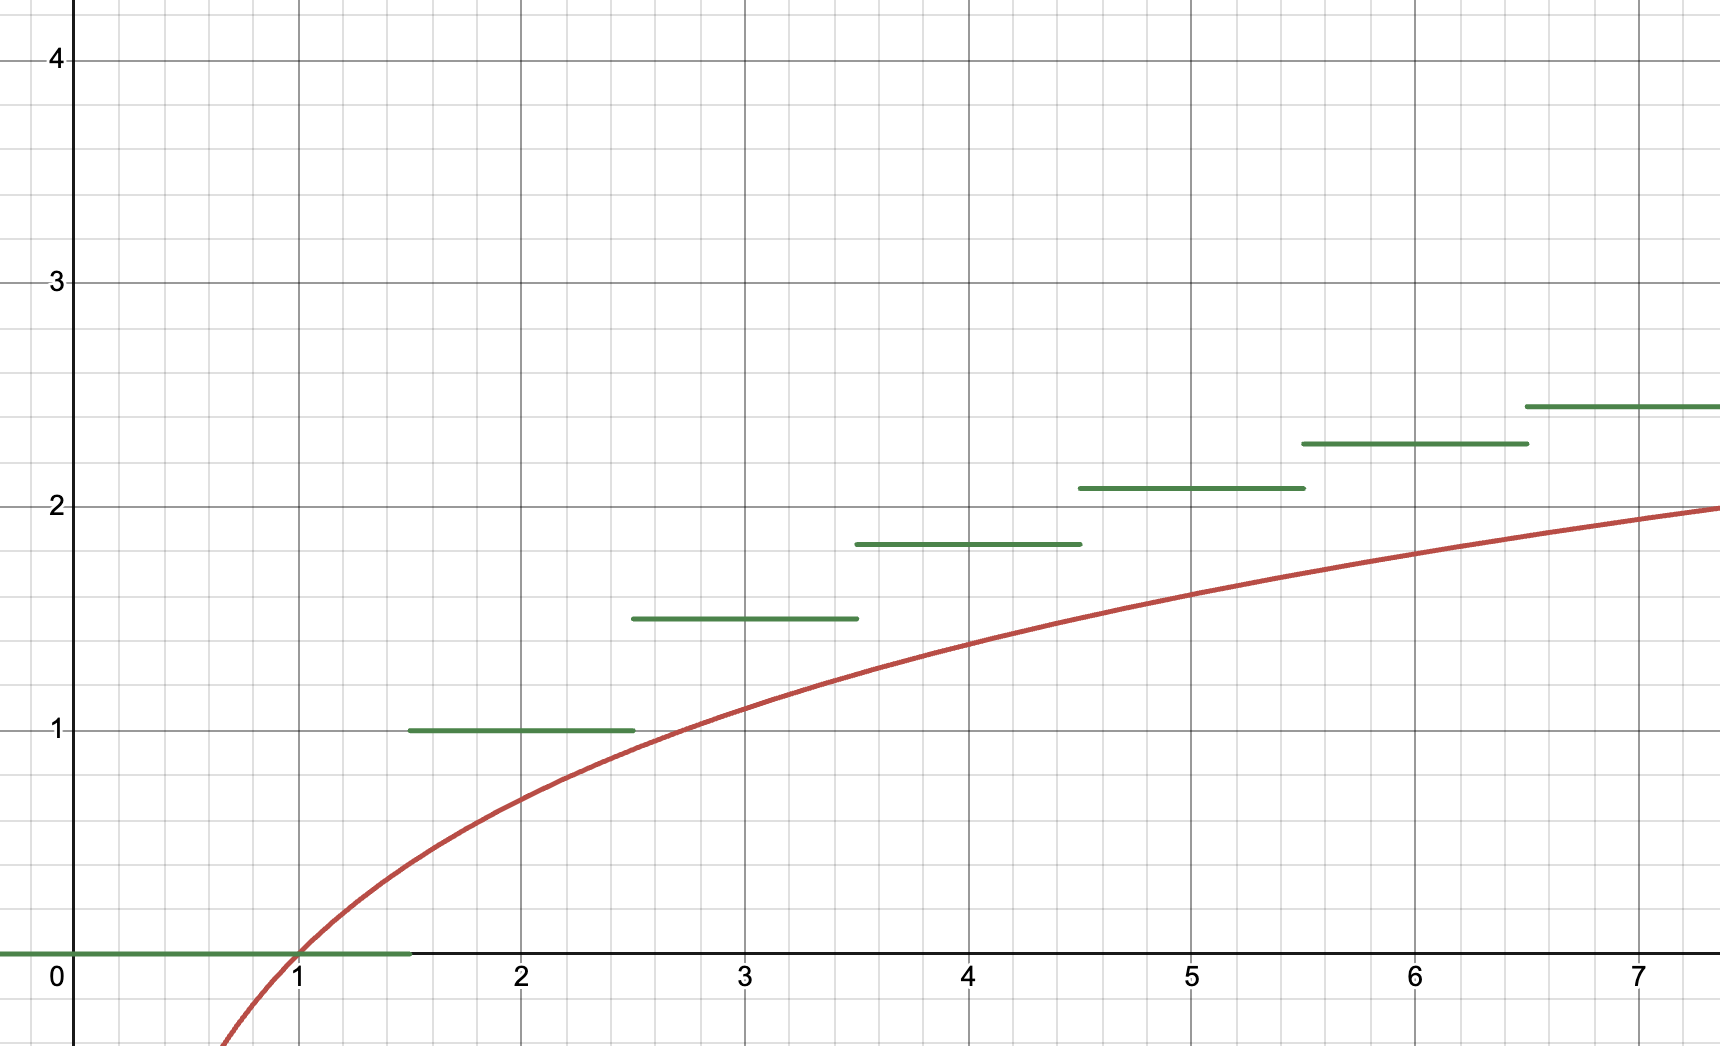
\includegraphics[width=0.7\linewidth]{Graph.png}
    \caption{Stochastic versus determenistic curve, note green is the stochastic one and red is determenistic. Graph made in desmos}
\end{figure}


\end{document}
